% dpplayne 30/10/15
% Game Engine Guide
\documentclass[a4paper, 10pt]{report}

\usepackage{graphicx}
\usepackage[T1]{fontenc}
\usepackage{textcomp}
\usepackage{listings}
\usepackage{color}

\definecolor{lightgrey}{rgb}{0.9,0.9,0.9}

%%% Change Chapter Head Style %%%
\makeatletter
\def\@makechapterhead#1{%
  %%%%\vspace*{50\p@}% %%% removed!
  {\parindent \z@ \raggedright \normalfont
    \ifnum \c@secnumdepth >\m@ne
        \huge\bfseries \@chapapp\space \thechapter
        \par\nobreak
        \vskip 2\p@
    \fi
    \interlinepenalty\@M
    \Huge \bfseries #1\par\nobreak
    \vskip 20\p@
  }}
\def\@makeschapterhead#1{%
  %%%%%\vspace*{50\p@}% %%% removed!
  {\parindent \z@ \raggedright
    \normalfont
    \interlinepenalty\@M
    \Huge \bfseries  #1\par\nobreak
    \vskip 40\p@
  }}
\makeatother
%%%%%


\lstset{language=Java}
\lstset{upquote=true}
\lstset{showstringspaces=false}
%\lstset{backgroundcolor=\color{lightgrey}}


\setlength{\parskip}{1em}
\setlength{\parindent}{0em}

\addtolength{\oddsidemargin}{-.8in}
\addtolength{\evensidemargin}{-.8in}
\addtolength{\textwidth}{1.60in}

\graphicspath{{Pictures/}}

% Title
\date{2023}
\title{\Huge {\bf 159.261 \\ Game Engine Programming Guide}}

% Author
\author{D.~Playne, A.~Leist, M.~Johnson \\ 
{\normalsize School of Mathematical and Computational Sciences}\\
{\normalsize Massey University}}

%Start the document
\begin{document}

%Put the title and author details into the report
\maketitle

%%Fill in with your abstract
%\begin{abstract}
%In this template we show how a report can be made easier in \LaTeX. Hopefully you find it helpful.
%\end{abstract}

%Print out a table of contents, comment out to remove.
%\tableofcontents

\chapter{Introduction}

The course examples, lab exercises and assignments in 159.261 are written in Java and make use of a simple game engine. This guide provides a simple introduction and explanation of how the game engine works and serves to complement the lectures with a reference.


\section*{Game Engine}

The game engine is implemented in the Java programming language in a file named {\tt GameEngine.java} and takes care of a number of the more complicated parts of writing a game. It also hides many of the object-oriented features of Java from you. You should note that this is not a good example of how to write a program in Java. It has been written this way to ease your transition from the introductory courses 159.101 and 159.102 that use the C++ programming language. This section will introduce you to how to use the game engine with a simple example.

The game engine takes care of creating and handling a window that appears on the screen as well as handling user input which can be optionally used by games. The engine can be used by simply creating a Java class (the name of the file must match the name of the class) that extends the game engine, this uses an object-oriented feature called inheritance (but don't worry about this).  The game class should have a main function that calls the function {\tt createGame}. The code to do this should be almost identical for every program based on the game engine (only the name of the class and file will change). An example of how to do this is shown in Listing~\ref{lst:SimpleGameSetup}.

\begin{lstlisting}[caption=Example showing a game called SimpleGame that uses GameEngine (must be written in a file named SimpleGame.java)., label=lst:SimpleGameSetup]
public class SimpleGame extends GameEngine {
    public static void main(String args[]) {
        createGame(new SimpleGame());
    }
    ...
}
\end{lstlisting}

When the game is first created, the GameEngine will call a function called {\tt init} that the game can use to initialise any variables for the game, set the size of the window etc. In our SimpleGame example there are no variables for the game so the {\tt init} function simply sets the size of the window to 500x500 - the size of the window can be changed by calling the GameEngine function {\tt setWindowSize(width,height)}. The {\tt init} function for SimpleGame is shown in Listing~\ref{lst:SimpleGame}

The GameEngine has an internal timer that will automatically call two functions that must be implemented by any game - {\tt update} and {\tt paintComponent}. The {\tt update} function is responsible for the dynamics of the game, this is where any changes to the state of the game should be written. The {\tt paintComponent} method is responsible for displaying the game on the screen. The GameEngine calls both of these functions multiple times per second based on the update rate or framerate of the game (usually 30 frames per second). A simple diagram of the flow of control for a game written using GameEngine can be seen in Figure~\ref{fig:GameEngineFlowControl}.

\begin{figure}[htbp]
\begin{center}
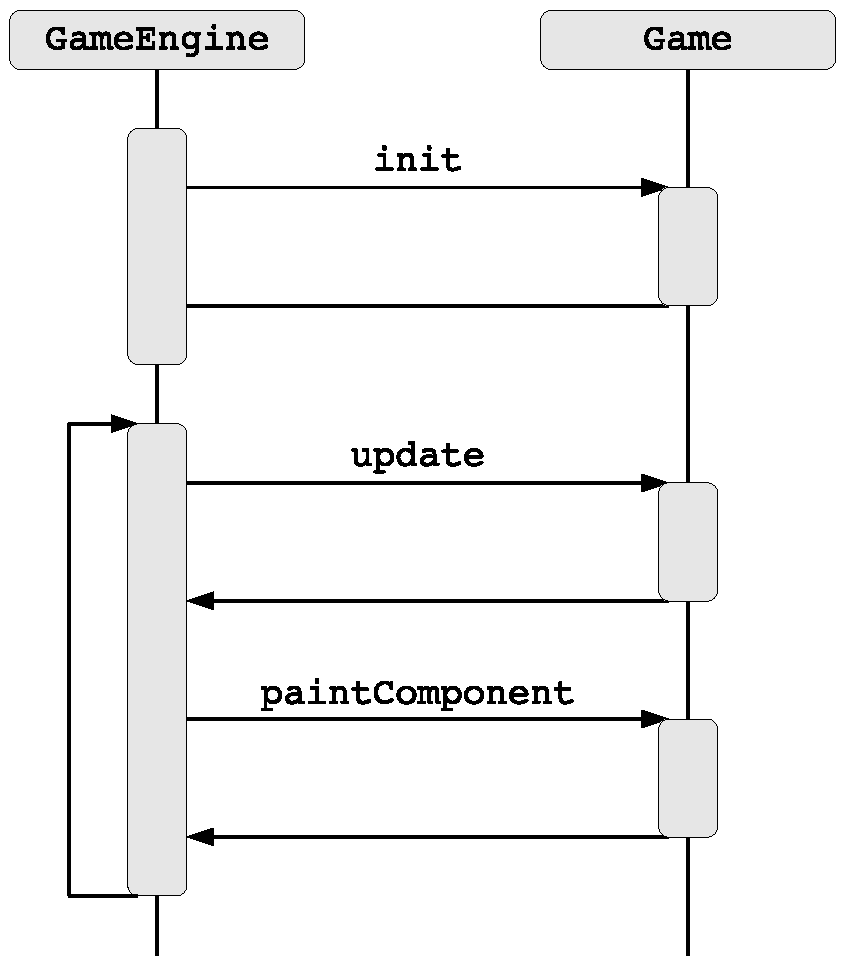
\includegraphics[width=0.4\textwidth]{GameEngine}
\caption{{\bf Flow control of a game based on GameEngine.}}
\label{fig:GameEngineFlowControl}
\end{center}
\end{figure}

In this simple example there is no game state and there are no dynamics (it is not really a game). The {\tt update} function does nothing but the paintComponent will use several functions from the GameEngine to draw the game on the screen. In this case, it simply draws a black background and then a white circle on the screen. The code for this is shown in Listing~\ref{lst:SimpleGame} and will produce the output shown in Figure~\ref{fig:SimpleGame}.

\begin{lstlisting}[caption=Initialisation function for SimpleGame., label=lst:SimpleGame]
public class SimpleGame extends GameEngine {
    public static void main(String args[]) {
        createGame(new SimpleGame());
    }
    public void init() {
        setWindowSize(500,500);
    }
    public void update(double dt) {
        
    }
    public void paintComponent() {
        changeBackgroundColor(black);
        clearBackground(500, 500);

        changeColor(white);
        drawCircle(100, 100, 50);
    }
}
\end{lstlisting}

\begin{figure}[htbp]
\begin{center}
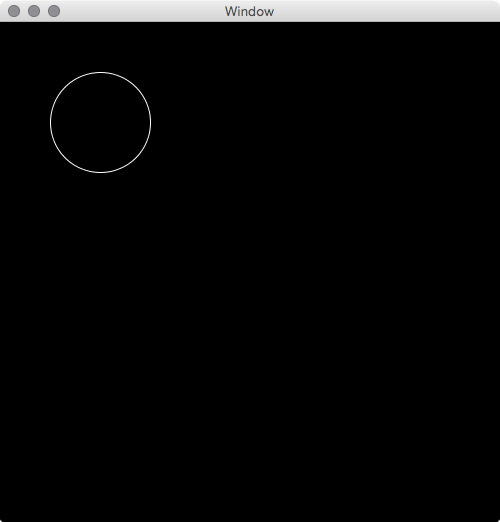
\includegraphics[width=0.5\textwidth]{SimpleGame}
\caption{{\bf Output on the screen of the SimpleGame example.}}
\label{fig:SimpleGame}
\end{center}
\end{figure}

% ---------------------------------------- Declaring Variables ----------------------------------------
\section*{Declaring Variables} \nonumber

There are no real global variables in Java but games written using this game engine can declare variables that will be accessible from any function in the game. Variables should be declared outside the functions (but still within the enclosing class) to make them available throughout the program. While the variables are declared outside functions, they should be assigned values in the {\tt init} function.

% ---------------------------------------- Init Function ----------------------------------------
\section*{Initialisation Function} \nonumber

The {\tt init} function is where any initialisation code should be performed. This function will only be called once before the game starts to run and is responsible for assigning values to all the variables in the game. Common operations performed in the {\tt init} function include: initialising variables to default or initial values, allocating memory for arrays, loading images from file and loading audio clips.

% ---------------------------------------- Update Function ----------------------------------------
\section*{Update Function} \nonumber

The {\tt update} function is where the main logic of the game is implemented. This function will be called many times per second (dependent on the framerate of the game) and receives a single parameter {\tt dt} that tells the function how much time has passed (in seconds) since the game was last updated ({\tt dt} is a double precision floating point number so it can measure fractions of a second). The {\tt dt} parameter can be used to ensure that the game objects move at the same rate irrespective of the actual framerate the game manages to achieve.

Common operations performed inside the {\tt update} function include moving game objects, checking for boundary conditions, checking for collisions between other objects etc.

% ---------------------------------------- paintComponent Function ----------------------------------------
\section*{PaintComponent Function} \nonumber

The {\tt paintComponent} function is where all of the code that draws objects on the screen belongs. This function should not try to move or update game objects and should only draw them on the screen. Code in this function will make heavy use of all of the drawing functions described in the following chapter.

% ---------------------------------------- Input Functions ----------------------------------------
\section*{Input Functions} \nonumber

The game engine supports a number of different input functions for receiving input from the mouse and/or the keyboard. These include pressing/releasing keys on the keyboard and mouse buttons as well as moving the mouse around on the screen. Use of these input functions allow the user to interact with the game and control certain game objects. Care should be taken that the logic inside an input function does not interfere with the game logic in the {\tt update} function.

% ---------------------------------------- Summary ----------------------------------------
\section*{Summary} \nonumber

This game engine provides a simple framework for developing 2D games with Java by providing some common functionality and abstracting away some unnecessary syntax. The main points to remember when writing a game using this game engine is where different code belongs. The previous sections describe where to declare variables, initialise variables, allocate memory, load images/audio files, update the game, draw objects on the screen and receive input from the user. The following section of this guide provides a detailed description of the functions the game engine provides and in some cases the common usage of the functions.



% ---------------------------------------- Game Engine Functions ----------------------------------------
\chapter{Game Engine Functions}

The following sections describe the major functions that the Java game engine provides for you to use.

If you look through the game engine source code you will discover that there are additional functions that relate to the internal workings of the game engine.

% ---------------------------------------- Window Functions ----------------------------------------
\section{Window Functions}

% ---------- setWindowSize ----------
{\large {\tt void setWindowSize(int width, int height)}}

Sets the useable size of the game window to {\tt (width, height)}. This function will automatically add the extra size need for the border around the window.


% ---------- width ----------
\hrulefill

{\large {\tt int width()}}

Returns the current width of the useable area of the game window. Allows games to avoid using hardcoded sizes that prevent the game from being scaled to different sizes.

% ---------- height ----------
\hrulefill

{\large {\tt int height()}}

Returns the current height of the useable area of the game window. Allows games to avoid using hardcoded sizes that prevent the game from being scaled to different sizes.

% ---------------------------------------- Drawing Functions ----------------------------------------
\section{Drawing Functions}

The following functions are used to draw the background and primitive shapes on the game engine frame. See the following Image Function section for details on loading and drawing images.

% ---------- changeBackgroundColor ----------
\hrulefill

{\large {\tt void changeBackgroundColor(Color c)}}

Usage: {\tt paintComponent()}

Sets the colour that the game engine will use to draw the background. Takes one parameter {\tt c} that must be one of the following pre-defined colours \{{\tt black, orange, cyan, pink, red, purple, blue, green, yellow, white}\}. Other colours can be used by calling the following method {\tt void changeBackgroundColor(int red, int green, int blue)} that allows a colour defined with rgb values.

% ---------- changeBackgroundColor ----------
\hrulefill

{\large {\tt void changeBackgroundColor(int red, int green, int blue)}}

Usage: {\tt paintComponent()}

Sets the colour that the game engine will use to draw the background. Takes three parameters {\tt red}, {\tt green}, {\tt blue} that are integers in the range [0, 255] that represent a colour in RGB space.

% ---------- clearBackground ----------
\hrulefill

{\large {\tt void clearBackground(int width, int height)}}

Usage: {\tt paintComponent()}

Clears the rectangle (0,0) to (width,height) to the current background colour of the game engine. This function is usually called at the beginning of the {\tt paintComponent()} with the width and height of the entire game panel. This will clear the entire screen to the background colour, the game graphics can then be drawn over the top of this background.

% ---------- changeColor ----------
\hrulefill

{\large {\tt void changeColor(Color c)}}

Usage: {\tt paintComponent()}

Sets the current drawing colour of the game engine. Any shape or text drawn following this call will be drawn with the colour {\tt c} (at least until the drawing colour is changed again). The parameter {\tt c} must be one of the following pre-defined colours \{{\tt black, orange, cyan, pink, red, purple, blue, green, yellow, white}\}. Other colours can be used by calling the following method {\tt void changeColor(int red, int green, int blue)} that allows a colour defined with rgb values. Transparent colours can be defined using {\tt Color c=new Color(red,green,blue,alpha)}. Where alpha is the transparency value (0-255).

% ---------- changeColor ----------
\hrulefill

{\large {\tt void changeColor(int red, int green, int blue)}}

Usage: {\tt paintComponent()}

Sets the current drawing colour of the game engine. Takes three parameters {\tt red}, {\tt green}, {\tt blue} that are integers in the range [0, 255] that represent a colour in RGB space.

% ---------- changeTransparency ----------
\hrulefill

{\large {\tt void changeTransparency(float alpha)}}

Usage: {\tt paintComponent()}

Sets the transparency for future drawImage() calls to alpha. 0.0=invisible 1.0=no transparency. 0.5=half transparent. Transparent image pixels are mixed with the existing window pixels using {\tt pixel=alpha * image\_pixel+(1-alpha) * window\_pixel }. 

% ---------- drawLine ----------
\hrulefill

{\large {\tt void drawLine(double x1, double y1, double x2, double y2)}}

Usage: {\tt paintComponent()}

Draws a line with the graphics context from the point {\tt (x1,y1)} to {\tt (x2, y2)}. The current drawing colour of the game engine will determine the colour of the line drawn.

% ---------- drawLine ----------
\hrulefill

{\large {\tt void drawLine(double x1, double y1, double x2, double y2, double l)}}

Usage: {\tt paintComponent()}

Draws a line with the graphics context from the point {\tt (x1,y1)} to {\tt (x2, y2)}. The width of the line is specified by the parameter {\tt l}. The current drawing colour of the game engine will determine the colour of the line drawn.

% ---------- drawRectangle ----------
\hrulefill

{\large {\tt void drawRectangle(double x, double y, double w, double h)}}

Usage: {\tt paintComponent()}

Draws a rectangle (only the outside lines) on the graphics context from the point {\tt (x,y)} with a width of {\tt w} and a height of {\tt h}. The current drawing colour of the game engine will determine the colour of the rectangle drawn.

% ---------- drawRectangle ----------
\hrulefill

{\large {\tt void drawRectangle(double x, double y, double w, double h, double l)}}

Usage: {\tt paintComponent()}

Draws a rectangle (only the outside lines) on the graphics context from the point {\tt (x,y)} with a width of {\tt w} and a height of {\tt h}. The width of the line is specified by the parameter {\tt l}. The current drawing colour of the game engine will determine the colour of the rectangle drawn.

% ---------- drawSolidRectangle ----------
\hrulefill

{\large {\tt void drawSolidRectangle(double x, double y, double w, double h)}}

Usage: {\tt paintComponent()}

Draws a solid or filled in rectangle on the graphics context from the point {\tt (x,y)} with a width of {\tt w} and a height of {\tt h}. The current drawing colour of the game engine will determine the colour of the rectangle drawn.

% ---------- drawCircle ----------
\hrulefill

{\large {\tt void drawCircle(double x, double y, double radius)}}

Usage: {\tt paintComponent()}

Draws a circle (only the outside line) on the graphics context centred at the point {\tt (x,y)} with a radius of {\tt radius}. The current drawing colour of the game engine will determine the colour of the circle drawn.

% ---------- drawCircle ----------
\hrulefill

{\large {\tt void drawCircle(double x, double y, double radius, double l)}}

Usage: {\tt paintComponent()}

Draws a circle (only the outside line) on the graphics context centred at the point {\tt (x,y)} with a radius of {\tt radius}. The width of the line is specified by the parameter {\tt l}. The current drawing colour of the game engine will determine the colour of the circle drawn.


% ---------- drawSolidCircle ----------
\hrulefill

{\large {\tt void drawSolidCircle(double x, double y, double radius)}}

Usage: {\tt paintComponent()}

Draws a solid or filled in circle on the graphics context centred at the point {\tt (x,y)} with a radius of {\tt radius}. The current drawing colour of the game engine will determine the colour of the circle drawn.

% ---------- drawPolygon ----------
\hrulefill

{\large {\tt void drawPolygon(GeneralPath polygon)}}

Usage: {\tt paintComponent()}

Draws the outline of a polygon using a predefined path. To create the polygon use: {\tt GeneralPath p=new GeneralPath();
p.moveTo(x1,y1);
p.lineto(x2,y2);
p.lineTo(x3,y3);
....
p.closePath();
} where (x1,x2),(y1,y2)... are the vertices of the polygon in clockwise order. The current drawing colour of the game engine will determine the colour of the polygon drawn.

% ---------- drawPolygon ----------
\hrulefill

{\large {\tt void drawPolygon(GeneralPath polygon, double l)}}

Usage: {\tt paintComponent()}

Draws the outline of a polygon using a predefined path and a line width of l. To create the polygon use: {\tt GeneralPath p=new GeneralPath();
p.moveTo(x1,y1);
p.lineto(x2,y2);
p.lineTo(x3,y3);
....
p.closePath();
} where (x1,x2),(y1,y2)... are the vertices of the polygon in clockwise order. The current drawing colour of the game engine will determine the colour of the polygon drawn.

% ---------- drawSolidPolygon ----------
\hrulefill

{\large {\tt void drawSolidPolygon(GeneralPath polygon)}}

Usage: {\tt paintComponent()}

Draws a filled polygon using a predefined path. To create the polygon use: {\tt GeneralPath p=new GeneralPath();
p.moveTo(x1,y1);
p.lineto(x2,y2);
p.lineTo(x3,y3);
....
p.closePath();
} where (x1,x2),(y1,y2)... are the vertices of the polygon in clockwise order. The current drawing colour of the game engine will determine the colour of the polygon drawn.


% ---------- drawText ----------
\hrulefill

{\large {\tt void drawText(double x, double y, String s)}}

Usage: {\tt paintComponent()}

Draw the text in the string {\tt s} on the graphics context with the bottom-left corner of the text at point {\tt (x,y)}. By default this function will draw the text in Arial font with a font size of 40. The current drawing colour of the game engine will determine the colour of the text drawn.

% ---------- drawBoldText ----------
\hrulefill

{\large {\tt void drawBoldText(double x, double y, String s)}}

Usage: {\tt paintComponent()}

Draw the text in the string {\tt s} on the graphics context with the bottom-left corner of the text at point {\tt (x,y)}. By default this function will draw the text in Arial bold font with a font size of 40. The current drawing colour of the game engine will determine the colour of the text drawn.


% ---------- drawText ----------
\hrulefill

{\large {\tt void drawText(double x, double y, String s, String font, int size)}}

Usage: {\tt paintComponent()}

Draw the text in the string {\tt s} on the graphics context with the bottom-left corner of the text at point {\tt (x,y)}. The font used to draw this text is defined by the parameter {\tt font} and the font-size by {\tt size}. The font specified must be supported by your system. The current drawing colour of the game engine will determine the colour of the text drawn.

% ---------- drawBoldText ----------
\hrulefill

{\large {\tt void drawBoldText(double x, double y, String s, String font, int size)}}

Usage: {\tt paintComponent()}

Draw the text in the string {\tt s} on the graphics context with the bottom-left corner of the text at point {\tt (x,y)}. The font used to draw this text will be bold and is defined by the parameter {\tt font} and the font-size by {\tt size}. The font specified must be supported by your system. The current drawing colour of the game engine will determine the colour of the text drawn.

% ---------------------------------------- Image Functions ----------------------------------------
\section{Image Functions}

The following functions can be used to load images from file, extract sub-images from a previously loaded image and draw images on the screen. These functions should be used to load images from file (usually in the {\tt init} function) and saved in an {\tt Image} variable. These images can then be drawn on the screen to represent various game objects using the {\tt drawImage} functions.

% ---------- loadImage ----------
\hrulefill

{\large {\tt Image loadImage(String filename)}}

Open the file specified by the parameter {\tt filename} and load the image contained within it. The image will be returned as an {\tt Image} variable that must be stored and can be drawn on the screen later using {\tt drawImage}.

% ---------- subImage ----------
\hrulefill

{\large {\tt Image subImage(Image image, int x, int y, int w, int h)}}

Extract a subsection of {\tt image} from (x,y) with size (w,h) and return it as a separate image. The coordinates {\tt x,y} and size {\tt w,h} are defined in pixels. This function is usually used to extract individual sprites from a sprite-sheet.

% ---------- drawImage ---------
\hrulefill

{\large {\tt void drawImage(Image image, double x, double y)}}

Usage: {\tt paintComponent()}

Draws the image defined by {\tt image} on the graphics context with the top-left corner at {\tt (x,y)}. The image will be drawn with the native size (in pixels) of the image. To draw the image larger/smaller than its original size use the following function {\tt void drawImage(Image image, double x, double y, double w, double h)}.

% ---------- drawImage ----------
\hrulefill

{\large {\tt void drawImage(Image image, double x, double y, double w, double h)}}

Usage: {\tt paintComponent()}

Draw the image defined by {\tt image} on the graphics context with the top-left corner at {\tt (x,y)}. The image will be drawn with a width of {\tt w} and a height of {\tt h}. Java will deal with scaling the image to the desired size.

% ---------------------------------------- Transform Functions ----------------------------------------
\section{Transform Functions}

The transform functions in GameEngine can transform the graphics context used to draw two-dimensional objects on the screen. These transforms are all affine transforms - they are linear transforms that preserve points and straight lines. Any set of lines that are parallel before an affine transform will remain parallel after it is applied. The supported transformations are - translate, rotate, scale and shear.

In addition to these transformations there are two functions for saving and restoring transforms. The {\tt saveCurrentTransform} will save the current transformation of the graphics context which can be restored later by calling the function {\tt restoreLastTransform}. These transforms are stored on a stack which is a first-in last-out data structure. This system allows multiple transforms to be saved, calling {\tt restoreLastTransform} will restore the saved transforms in the reverse order they were added. It is important to note that all transforms will be reset between frames. The transform will be reset to a default before each call to {\tt paintComponent}.

% ---------- saveCurrentTransform ----------
\hrulefill

{\large {\tt void saveCurrentTransform()}}

Usage: {\tt paintComponent()}

Saves the current transform of the graphics context and adds it to the stack of saved transforms. General usage is to save the current transform before drawing an object and then restoring it afterwards.

% ---------- restoreLastTransform ----------
\hrulefill

{\large {\tt void restoreLastTransform()}}

Usage: {\tt paintComponent()}

Restores the most recently saved transform of the graphics context and removes it from the stack. Repeatedly calling this function will cycle the graphics context through all of the saved transforms in the reverse order they were saved in.

% ---------- translate ----------
\hrulefill

{\large {\tt void translate(double x, double y)}}

Usage: {\tt paintComponent()}

Applies a translation to the graphics context. This transform moves the graphics context by {\tt (x,y)} pixels in the x- and y-dimensions respectively. This translation will occur within the coordinate space of the existing graphics context, previous transformations will have an effect on the transformation. An example of this transform is shown in Figure~\ref{fig:Translate}.

\begin{figure}[htbp]
\begin{center}
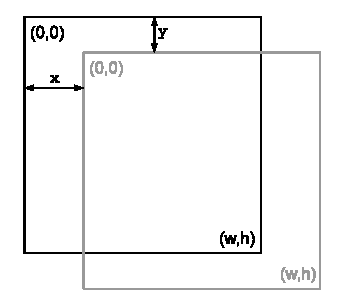
\includegraphics[width=0.3\textwidth]{translation}
\caption{{\bf Example of a translation transformation.}}
\label{fig:Translate}
\end{center}
\end{figure}

% ---------- rotate ----------
\hrulefill

{\large {\tt void rotate(double a)}}

Usage: {\tt paintComponent()}

Applies a rotation to the graphics context. The rotation transformation will rotate the graphics context by {\tt a} degrees around the origin {\tt (0,0)}. An example of how this transformation works can be seen in Figure~\ref{fig:Rotate}.

\begin{figure}[htbp]
\begin{center}
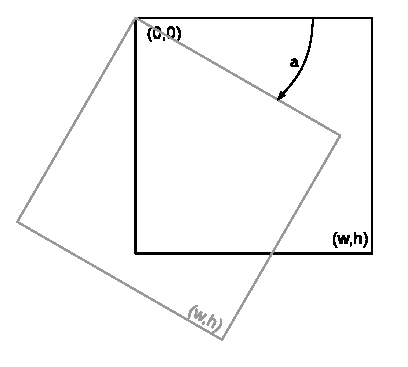
\includegraphics[width=0.3\textwidth]{rotation}
\caption{{\bf Example of a rotation transformation.}}
\label{fig:Rotate}
\end{center}
\end{figure}

% ---------- scale ----------
\hrulefill

{\large {\tt void scale()}}

Usage: {\tt paintComponent()}

Applies a scale transformation to the graphics context. This will scale the graphics context by a factor of {\tt (x,y)} in the x- and y-dimensions respectively. Figure~\ref{fig:Scale} shows an example of the scale transform.

\begin{figure}[h!]
\begin{center}
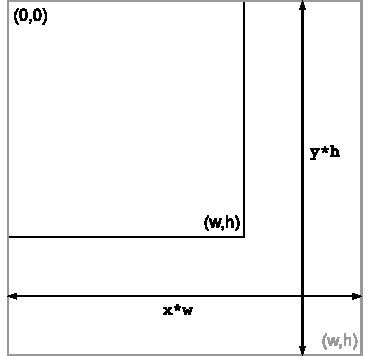
\includegraphics[width=0.3\textwidth]{scale}
\caption{{\bf Example of a scale transformation.}}
\label{fig:Scale}
\end{center}
\end{figure}

% ---------- shear ----------
\hrulefill

{\large {\tt void shear()}}

Usage: {\tt paintComponent()}

Applies a shear transformation to the graphics context. This will apply a shear of {\tt (x,y)} in the x- and y-dimensions respectively. An example of this shear transform is shown in Figure~\ref{fig:Shear}.

\begin{figure}[h!]
\begin{center}
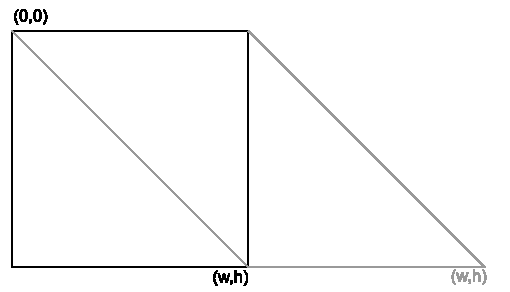
\includegraphics[width=0.35\textwidth]{shear}
\caption{{\bf Example of a shear transformation.}}
\label{fig:Shear}
\end{center}
\end{figure}

\hrulefill

% ---------- Transform Usage ----------
\subsection*{Common Transform Usage} \nonumber

The most common usage of graphics transforms in games is for drawing objects with a given position and rotation. For example drawing the spaceship from the Lab exercises. An important part process is to save the current transform before drawing and to restore it at the end of the process. This ensures that the transforms used to draw one object do not affect any others. After the transform is saved, a translation is applied to move the graphics context to the centre of where the object should be drawn. Then a rotation is applied to rotate the context to the desired angle, the rotation is always applied around the point {\tt (0,0)}. Finally the object is drawn centred around the point {\tt (0,0)}. For example, if an image is 60x60 pixels, it will be drawn at the point {\tt (-30, -30)} to {\tt (30, 30)}. The process for drawing an object at the position {\tt (x,y)} with a rotation {\tt a} is shown in Figure~\ref{fig:Object-Draw}.


\begin{figure}[htbp]
\begin{center}
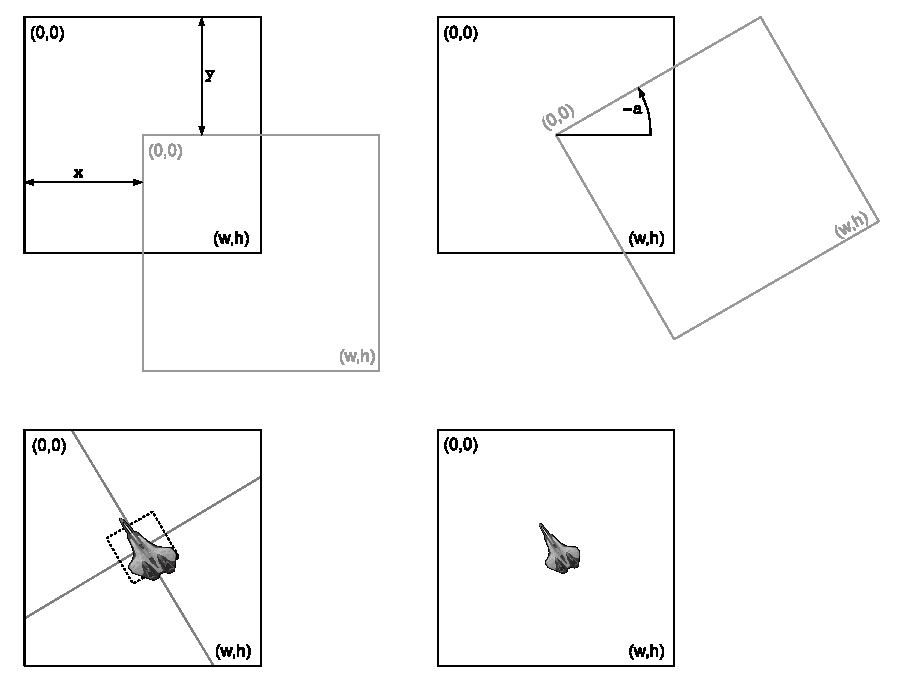
\includegraphics[width=0.80\textwidth]{Object}
\caption{ Transforms used to draw an object centred at position {\tt (x,y)} with rotation {\tt a}. First the current transform is saved (not shown), the graphics context is translated to position {\tt (x,y)} (top-left), the context is rotated by angle {\tt a} (top-right), the object is drawn (bottom-left) and finally the saved transform is restored (bottom-right). Sprites were made by MillionthVector (millionthvector.blogspot.co.nz) and are licensed under a Creative Commons Attribution 4.0 International License.}
\label{fig:Object-Draw}
\end{center}
\end{figure}
\vspace{2em}

% ---------------------------------------- Input Functions ----------------------------------------
\section{Input Functions}

The input functions in the game engine are called automatically whenever an input event occurs. There are a whole set of different input events that can occur and will cause the matching input function to be called. For example, whenever the user presses a key down on the keyboard, the game engine will call the {\tt keyPressed(KeyEvent event)} function. If you have not written an implementation of this function in your game, nothing will happen. If you have written an implementation then the function will be called and your game can respond to input.

The input functions will receive a single parameter which is either a {\tt KeyEvent} for keyboard functions or a {\tt MouseEvent} for mouse functions. These parameters can be used to determine information about the event that occurred such as the position of the mouse or which key was actually pressed. Each of the functions are described in more detail as follows.

% ---------- keyPressed ----------
\hrulefill

{\large {\tt void keyPressed(KeyEvent event)}}

Usage: Called automatically whenever the user presses a key on the keyboard. See the following section {\tt KeyEvent} for details on how to extract information from a keyboard event.

% ---------- keyReleased ----------
\hrulefill

{\large {\tt void keyReleased(KeyEvent event)}}

Usage: Called automatically whenever the user releases a key on the keyboard. See the following section {\tt KeyEvent} for details on how to extract information from a keyboard event.	

% ---------- keyTyped ----------
\hrulefill

{\large {\tt void keyTyped(KeyEvent event)}}

Called automatically whenever the user presses and immediately releases a key on the keyboard. See the following section {\tt KeyEvent} for details on how to extract information from a keyboard event.

% ---------- KeyEvent ----------
\hrulefill

{\large {\tt KeyEvent event}}

The {\tt KeyEvent} parameter sent to the keyboard events contains information about the keyboard event that has just occurred. The main information needed from the event is which key was pressed/released/typed. For the {\tt keyPressed} and {\tt keyReleased} events, the information can be obtained by calling {\tt event.getKeyCode()}. Calling this function will return an integer key code representing the key that can then be compared to a set of key codes to determine which key it represents. Some examples of key codes are the up-arrow {\tt KeyEvent.VK\_UP}, the spacebar {\tt KeyEvent.VK\_SPACE} and the enter key {\tt KeyEvent.VK\_ENTER}.

The {\tt keyTyped} is higher-level function and uses the function {\tt event.getKeyChar()} to extract the information of which key was pressed. Key typed events are not generated for keys that don't generate Unicode characters (action keys, modifier keys, etc).

For a complete list see:

http://docs.oracle.com/javase/7/docs/api/java/awt/event/KeyEvent.html

\hrulefill

% ---------- Keyboard Usage ----------
\subsection*{Common Keyboard Function Usage} \nonumber

The following code segment (Listing:~\ref{lst:KeyExample}) shows an example of a keyboard input function that prints a message whenever the spacebar or enter key is pressed.

\vspace{1em}
\begin{lstlisting}[caption=Example use of the keyPressed function and the KeyEvent., label=lst:KeyExample]
public void keyPressed(KeyEvent event) {
   if(event.getKeyCode() == KeyEvent.VK_SPACE) {
      System.out.println("Space Bar");
   } else if(event.getKeyCode() == KeyEvent.VK_ENTER) {
      System.out.println("Enter Key");
   }
}
\end{lstlisting}

% ---------- mousePressed ----------
\hrulefill

\vspace{1em}

{\large {\tt void mousePressed(MouseEvent event)}}

Called automatically whenever the user presses a mouse button. See the following section {\tt MouseEvent} for details on how to extract information from a mouse event.

% ---------- mouseReleased ----------
\hrulefill

{\large {\tt void mouseReleased(MouseEvent event)}}

Called automatically whenever the user releases a mouse button. See the following section {\tt MouseEvent} for details on how to extract information from a mouse event.

% ---------- mouseClicked ----------
\hrulefill

{\large {\tt void mouseClicked(MouseEvent event)}}

Called automatically whenever the user presses and immediately releases a mouse button. See the following section {\tt MouseEvent} for details on how to extract information from a mouse event. Be careful using this callback to detect mouse clicks because it will not be called if the user clicks the mouse button and then moves the mouse before releasing it. 

% ---------- mouseEntered ----------
\hrulefill

{\large {\tt void mouseEntered(MouseEvent event)}}

Called automatically whenever the mouse cursor enters the game window. See the following section {\tt MouseEvent} for details on how to extract information from a mouse event.

% ---------- mouseExited ----------
\hrulefill

{\large {\tt void mouseExited(MouseEvent event)}}

Called automatically whenever the mouse cursor exits the game window. See the following section {\tt MouseEvent} for details on how to extract information from a mouse event.

% ---------- mouseMoved ----------
\hrulefill

{\large {\tt void mouseMoved(MouseEvent event)}}

Called automatically whenever the user moves the mouse (inside the game window). See the following section {\tt MouseEvent} for details on how to extract information from a mouse event.

% ---------- mouseDragged ----------
\hrulefill

{\large {\tt void mouseDragged(MouseEvent event)}}

Called automatically whenever the user moves the mouse (inside the game window) while holding down a mouse button. See the following section {\tt MouseEvent} for details on how to extract information from a mouse event.

% ---------- MouseEvent ----------
\hrulefill

{\large {\tt MouseEvent event}}

The {\tt Mouse} parameter sent to the mouse event functions contains information about the mouse event that has just occurred. The main information needed from the event is which mouse button was pressed/released (if any) and where the mouse is. The mouse button pressed can be obtained by calling {\tt event.getButton()} which will return an integer code for the mouse button. This can be compared to the values \\{\tt MouseEvent.BUTTON1}, {\tt MouseEvent.BUTTON2} and {\tt MouseEvent.BUTTON3} to determine which mouse button was used in the event.

The current position of the mouse cursor (in the game window) can be determined by calling the functions {\tt event.getX()} and {\tt event.getY()} that return the x and y coordinates of the cursor respectively. An example of a common mouse event function is shown in the following section.

\hrulefill

% ---------- Mouse Usage ----------
\subsection*{Common Mouse Function Usage} \nonumber

The following code segment (Listing:~\ref{lst:MouseExample}) shows an example of a mouse input function that prints out which mouse button was just pressed and where the mouse cursor is on the window.

\vspace{1em}
\begin{lstlisting}[caption=Example use of the mousePressed function and the MouseEvent., label=lst:MouseExample]
public void mousePressed(MouseEvent event) {
   if(event.getButton() == MouseEvent.BUTTON1) {
      System.out.println("Mouse Button 1 pressed");
   } else if(event.getButton() == MouseEvent.BUTTON2) {
      System.out.println("Mouse Button 2 pressed");
   } else if(event.getButton() == MouseEvent.BUTTON3) {
      System.out.println("Mouse Button 3 pressed");
   }
   int x = event.getX();
   int y = event.getY();
   
   System.out.println(" at position(" + x + "," + y + ")");
}
\end{lstlisting}
\vspace{1em}

% ---------------------------------------- Audio Functions ----------------------------------------
\section{Audio Functions}

The game engine provides a set of functions for loading and playing audio files. The game engine is limited in the type and size of the audio files it can play. The engine should support {\tt .wav} files. Audio files can be played with two main functions - {\tt playAudio} and {\tt startAudioLoop}. The function {\tt playAudio} will play an audio clip once after which it will stop. This function can be called many times and have many version of the same audio clip playing at once. The {\tt startAudioLoop} function will start the audio clip playing on a continuous loop, only one loop of an audio clip can be playing at once. These (and additional) audio functions are described below:

% ---------- loadAudio ----------
\hrulefill

{\large {\tt AudioClip loadAudio(String filename)}}

Opens the file specified by {\tt filename} and loads the audio clip information from it. Returns an {\tt AudioClip} that can be stored and used to play the audio later.

% ---------- playAudio ----------
\hrulefill

{\large {\tt void playAudio(AudioClip audioClip)}}

Plays the audio clip specified by the parameter {\tt audioClip} with a default volume setting. The clip will be played once and will then stop.

% ---------- playAudio ----------
\hrulefill

{\large {\tt void playAudio(AudioClip audioClip, float volume)}}

Plays the audio clip specified by the parameter {\tt audioClip} with a volume specified by the parameter {\tt volume}. Note that the volume is specified in decibels. The clip will be played once and will then stop.

% ---------- startAudioLoop  ----------
\hrulefill

{\large {\tt void startAudioLoop(AudioClip audioClip)}}

Starts the audio clip specified by the parameter {\tt audioClip} playing on a continuous loop. The clip can be stopped by calling the function {\tt stopAudioLoop} and passing the same audio clip.

% ---------- startAudioLoop  ----------
\hrulefill

{\large {\tt void startAudioLoop(AudioClip audioClip, float volume)}}

Starts the audio clip specified by the parameter {\tt audioClip} playing on a continuous loop with a volume specified by the parameter {\tt volume}. The clip can be stopped by calling the function {\tt stopAudioLoop} and passing the same audio clip.

% ---------- stopAudioLoop ----------
\hrulefill

{\large {\tt void stopAudioLoop(AudioClip audioClip)}}

Stops the audio clip specified by the parameter {\tt audioClip} from playing on continuous loop.

% ---------- Audio Usage ----------
\subsection*{Common Audio Function Usage} \nonumber

The code snippet in Listing~\ref{lst:audio} shows the common usage of loading and playing an audio file.

\vspace{1em}
\begin{lstlisting}[caption=Example use game engine audio functions., label=lst:audio]
...
AudioClip beep;
AudioClip background;

public void init() {
   ...
   beep = loadAudio("beep.wav");
   background = loadAudio("background.wav");
   
   startAudioLoop(background);
}


public void mousePressed(MouseEvent event) {
   if(event.getButton() == MouseEvent.BUTTON1) {
      playAudio(beep);
   }
}
....
\end{lstlisting}


\vspace{1em}

% ---------------------------------------- Maths Functions ----------------------------------------
\section{Mathematical Functions}

The game engine provides the following functions for performing common Mathematics operations. Trigonometry functions are described in the following section.

% ---------- rand ----------
\hrulefill

{\large {\tt int rand(int max)}}

Generates a uniform random value and converts it to an integer in the range [0, max). Integers starting from (and including) zero up to (but not including) {\tt max} will be returned with an equal probability.

% ---------- rand ----------
\hrulefill

{\large {\tt float rand(float max)}}

Generates a single-precision uniform random value in the range [0, max).

% ---------- rand ----------
\hrulefill

{\large {\tt double rand(double max)}}

Generates a double-precision uniform random value in the range [0, max).

% ---------- floor ----------
\hrulefill

{\large {\tt int floor(double value)}}

Converts a double value to an integer by returning the largest integer that is less than or equal to the parameter {\tt value}.

% ---------- ceil ----------
\hrulefill

{\large {\tt int ceil(double value)}}

Converts a double value to an integer by returning the smallest integer that is greater than than or equal to the parameter {\tt value}.

% ---------- round ----------
\hrulefill

{\large {\tt int round(double value)}}

Converts a double value to an integer by rounding the parameter {\tt value} to the closest integer.

% ---------- abs ----------
\hrulefill

{\large {\tt int abs(int value)}}

Calculates the absolute value of the integer {\tt int} parameter {\tt value}. Absolute value removes the sign of a value.

% ---------- abs ----------
\hrulefill

{\large {\tt float abs(float value)}}

Calculates the absolute value of the single-precision {\tt float} parameter {\tt value}. Absolute value removes the sign of a value.

% ---------- abs ----------
\hrulefill

{\large {\tt double abs(double value)}}

Calculates the absolute value of the double-precision {\tt double} parameter {\tt value}. Absolute value removes the sign of a value.

% ---------- sqrt ----------
\hrulefill

{\large {\tt double sqrt(double value)}}

Calculates the square root of the parameter {\tt value}.

% ---------- length ----------
\hrulefill

{\large {\tt double length(double x, double y)}}

Calculates the length of the vector (x,y). This is the same as the distance from the point (0,0) to the point (x,y).

% ---------- distance ----------
\hrulefill

{\large {\tt double distance(double x1, double y1, double x2, double y2)}}

Calculates the distance from the point (x1,y1) to the point (x2,y2).

% ---------------------------------------- Trigonometry Functions ----------------------------------------
\section{Trigonometry Functions}

The game engine provides the following Trigonometry functions. All trig functions take and return values specified in degrees. The methods {\tt toDegrees} and {\tt toRadians} can be used to convert between radians and degrees if necessary.

% ---------- toDegrees ----------
\hrulefill

{\large {\tt double toDegrees(double radians)}}

Converts the parameter {\tt radians} from an angle specified in radians to the same angle specified in degrees.

% ---------- toRadians ----------
\hrulefill

{\large {\tt double toDegrees(double degrees)}}

Converts the parameter {\tt degrees} from an angle specified in degrees to the same angle specified in radians.

% ---------- cos ----------
\hrulefill

{\large {\tt double cos(double value)}}

Calculates the cosine of the parameter {\tt value}.

% ---------- acos ----------
\hrulefill

{\large {\tt double acos(double value)}}

Calculates the inverse cosine or arccosine of the parameter {\tt value}. Parameter must be in the range [-1,1].

% ---------- sin ----------
\hrulefill

{\large {\tt double sin(double value)}}

Calculates the sine of the parameter {\tt value}.

% ---------- asin ----------
\hrulefill

{\large {\tt double asin(double value)}}

Calculates the inverse sine or arcsine of the parameter {\tt value}. Parameter must be in the range [-1,1].

% ---------- tan ----------
\hrulefill

{\large {\tt double tan(double value)}}

Calculates the tangent of the parameter {\tt value}. Result is not defined for values [$90^{\circ}, 270^{\circ}, 450^{\circ}$...] 

% ---------- atan ----------
\hrulefill

{\large {\tt double atan(double value)}}

Calculates the inverse tangent or arctangent of the parameter {\tt value}. 

% ---------- atan2 ----------
\hrulefill

{\large {\tt double atan2(double x, double y)}}

Returns the angle theta from the conversion of rectangular coordinates (x, y) to polar coordinates (r, theta).

% ---------- Examples ----------
%\chapter{Examples}



\end{document}

